\mathchardef\period=\mathcode`.
\documentclass[a4paper]{article}
\usepackage[top=1.45cm, bottom=1cm, left=1cm, right=1cm]{geometry}

\usepackage{parskip} % Package to tweak paragraph skipping
\usepackage{tikz} % Package for drawing
\usepackage{tkz-euclide}
\usepackage{siunitx}
\usepackage{wrapfig}
\usepackage{graphicx}

\usetikzlibrary{fit,positioning}
\usetikzlibrary{arrows.meta}
\usetikzlibrary{patterns,patterns.meta}
\usepackage[inline]{enumitem}
\usepackage{amsmath,amssymb}
\usepackage{tasks}
\usepackage{amsmath}
\usepackage{hyperref}
\usepackage[main=lithuanian, german, shorthands=off]{babel}
\usepackage{tgpagella}
\usepackage[L7x,T1]{fontenc}
\usepackage[utf8]{inputenc}
\usepackage{enumitem}
\usepackage{booktabs} % For better looking tables
\usepackage{venndiagram}
\usepackage{subfig}
\usepackage{multirow}
\usepackage{tabularray}
\usepackage{lipsum}
\usepackage{fancyhdr}

\usepackage{blindtext}
\usepackage{adjustbox}
\AfterEndEnvironment{wrapfigure}{\setlength{\intextsep}{0mm}}
\usepackage{afterpage}

\usepackage{icomma}

% Header | Footer 
\fancyhf{} % clear all header and footer fields
\fancyhead[R]{pusmečio pabaiga | kontrolinis darbas}
% L for Left, you can also use R for Right or C for Center
\fancyfoot[R]{pusmečio pabaiga | kontrolinis darbas}

% L for Left, you can also use R for Right or C for Center
\setlength{\headheight}{0.5pt} % Adjust the head height
\renewcommand{\headrulewidth}{0.4pt} % Line under the header
\renewcommand{\footrulewidth}{0.4pt} % Line above the footer
% Header | Footer 

\newcommand{\germanqq}[1]{{\selectlanguage{german}\glqq#1\grqq\selectlanguage{english}}}

\DeclareMathOperator{\tg}{tg}
\newcommand{\tgx}{\tg x}

\DeclareMathOperator{\arctg}{arctg}
\newcommand{\arctgx}{\arctg x}

\makeatletter
\newcommand*{\rom}[1]{\expandafter\@slowromancap\romannumeral #1@}
\makeatother

\title{Kontrolinis darbas - progresijos}
\author{Vilius Paliokas}
\date{2023/10/17}

\setlist{after=\vspace{\baselineskip}}

% Title spacing
\usepackage{titlesec}
\titlespacing*{\subsection}{0pt}{\baselineskip}{0.5\baselineskip}
% ------------------------ 

\newcommand\blankpage{%
      \null
      \thispagestyle{empty}%
      \addtocounter{page}{-1}%
      \newpage}

\begin{document}
\thispagestyle{fancy}

\titlespacing*{\subsection}{0pt}{.75ex}{0.75ex}

\subsection*{3 variantas}

\begin{enumerate}
      \item \textit{(1 taškas)} Kuri funkcija nelyginė?
            \begin{tasks}[item-format={\normalfont}, after-item-skip=2mm,
                        label=\Alph*, label-format={\bfseries}](4)
                  \task $f(x)=-x^3-3$
                  \task $g(x)=\sqrt[3]{x-3}$
                  \task $h(x)=-3x^3$
                  \task $t(x)=\frac{1}{x-3}$
            \end{tasks}

      \item \textit{(1 taškas)} Kurios funkcijos grafikas pavaizduotas 1 pav.?
            \begin{tasks}[item-format={\normalfont}, after-item-skip=2mm,
                        label=\Alph*, label-format={\bfseries}](4)
                  \task $f(x)=\log_{\frac{1}{2}}(x+\frac{1}{2})$
                  \task $f(x)=2^x$
                  \task $f(x)=(\frac{1}{2})^x$
                  \task $f(x)=\log_{2}(x+2)$
            \end{tasks}

      \item \textit{(1 taškas)} Kuriame intervale didėja funkcijos
            $f(x)=\sin(x+90^\circ)$ reikšmės?
            \begin{tasks}[item-format={\normalfont}, after-item-skip=2mm,
                        label=\Alph*, label-format={\bfseries}](4)
                  \task $(135^\circ; 270^\circ)$
                  \task $(-270^\circ; 180^\circ)$
                  \task $(540^\circ; 720^\circ)$
                  \task $(-90^\circ; 90^\circ)$
            \end{tasks}

      \item \textit{(1 taškas)} Kokia didžiausia ir mažiausia $f(x)=6-4\cos{x}$
            reikšmės?
            \vspace{7mm}

      \item \textit{(1 taškas)} Taškas $(5; 32)$ yra funkcijos $f(x)=a^x$
            grafiko taškas. Raskite \underline{$a$ reikšmę}.
            \vspace{7mm}

      \item \textit{(1 taškas)} Taškas $(5; 32)$ yra funkcijos $f(x)=a^x$
            grafiko taškas. Raskite \underline{$f(-4)$ reikšmę}.
            \vspace{7mm}

      \item \textit{(1 taškas)} Kiek susikirtimo taškų turi $f(x)=-x^2-2$ ir
            $g(x)=0$ grafikai?
            \vspace{7mm}

      \item \textit{(1 taškas)} Funkcijos $y=f(x)$ apibrėžimo sritis $D(f)=[-5;
                  12)$, reikšmių sritis $E(f)=[-1;3]$. Nustatykite funkcijos
            $y=g(x)=3-f(x+3)$
            \underline{apibrėžimo sritį}.
            \vspace{7mm}

      \item \textit{(1 taškas)} Funkcijos $y=f(x)$ apibrėžimo sritis $D(f)=[-5;
                  12)$, reikšmių sritis $E(f)=[-1;3]$. Nustatykite funkcijos
            $y=g(x)=3-f(x+3)$
            \underline{reikšmių sritį}.
            \vspace{7mm}

      \item \textit{(1 taškas)} Kuriems koordinačių plokštumos ketvirčiams
            priklauso funkcijos $y=f(x)=-\sqrt[3]{x-1}+1$ grafiko taškai?
            \vspace{7mm}

      \item \textit{(1 taškas)} 2 paveiksle pavaizduotas funkcijos
            $f(x)=\frac{4}{x+m}+n$ grafikiko eskizas. Raskite $m$ ir $n$
            reikšmes.
            \vspace{7mm}


            \begin{figure}[!htpb]
                  \centering
                  \begin{minipage}[]{0.5\linewidth}
                        \centering

                        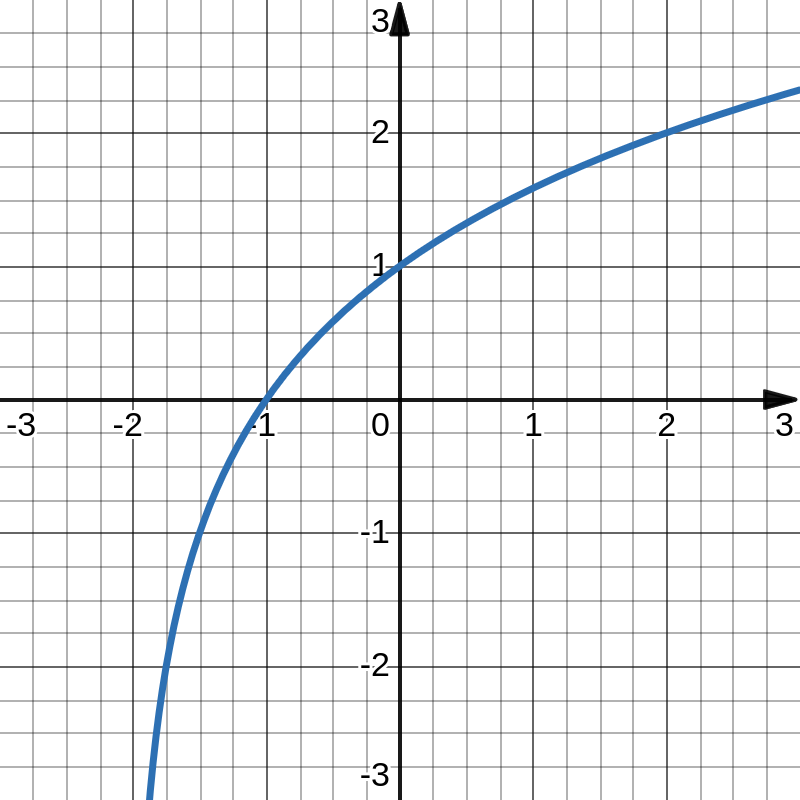
\includegraphics[width=0.5\linewidth]{images/func_1.png}
                        \captionof{figure}{A figure}
                        \label{fig:test1}
                  \end{minipage}%
                  \begin{minipage}{.5\textwidth}
                        \centering
% https://www.desmos.com/calculator/kgs889clek
                        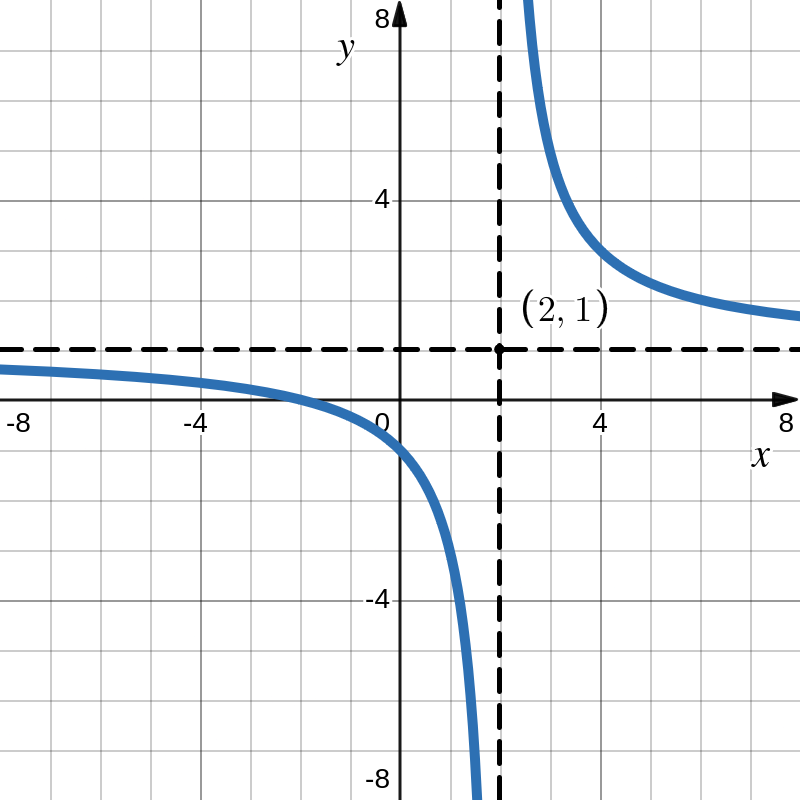
\includegraphics[width=0.5\linewidth]{images/func_2.png}
                        \captionof{figure}{Another figure}
                        \label{fig:test2}
                  \end{minipage}
            \end{figure}
\end{enumerate}

\begin{small}
      \begin{enumerate*}[label={(\arabic*)}, topsep=0pt, partopsep=0pt]
            \item \textbf{Visur}, išskyrus įrodymus, \textbf{užrašykite
                  atsakymus} ($Ats\ldots$);
            \item Jokio sukčiavimo. Negalima naudotis užrašais, vadovėliais,
            elektroniniais prietaisais;
            \item Jokio kalbėjimo;
            \item Rašyti aiškiai, nedviprasmiškai;
            \item Galima naudotis tik savo skaičiuotuvu ir formulių lapu;
      \end{enumerate*}
\end{small}

\pagenumbering{gobble}

\def\width{19}
\def\hauteur{28}

\begin{tikzpicture}[x=1cm, y=1cm, semitransparent]
      % \draw[step=1mm, line width=0.1mm, black!30!white] (0,0) grid (\width,\hauteur);
      \draw[step=4mm, line width=0.2mm, black!60!white] (0,0) grid
      (\width,\hauteur);
      % \draw[step=5cm, line width=0.5mm, black!50!white] (0,0) grid (\width,\hauteur);
      % \draw[step=1cm, line width=0.3mm, black!90!white] (0,0) grid (\width,\hauteur);
\end{tikzpicture}
\end{document}